\documentclass[fontsize=9pt,paper=A6,twoside,BCOR=1mm,DIV=22,headinclude]{scrarticle}
\usepackage{breviarium}
\begin{document}
\titulum{Breviarium Monasticum}{In Festo Pentecostes}{Officium in die}

%\vspace{-1.5em}

\begin{multicols}{2}
\dieii{Feria VI}{Post Octavam Ascensionis}{}{Semiduplex}

\hora{Ad Vesperas}

\rubric{\A ut in Laudibus sequentis diei, Psalmi de Dominica.}

\rubric{Capitulum ut infra ad Laudes seq. diei.}

\Rbr Ascéndens Christus in altum, \red{*} Allelúja, allelúja.
\red{A}scéndens.
\V Captívam duxit captivitátem.
\red{A}llelúja.
\red{G}lória Patri.
\red{A}scéndens.

\rubric{Hymnus \black{Jesu, nostra redémptio,} ut infra.}

\V Dóminus in cælo, allelúja.
\R Parávit sedem suam, allelúja.

\M Hæc locútus sum f vobis, ut cum vénerit hora eórum, reminiscámini quia ego dixi vobis, allelúja.

\rubric{Oratio ut infra ad Laudes.}

\dieii{Sabbato}{In Vigilia Pentecostes}{}{Semiduplex I classis}

\hora{Ad Laudes}
\etper
\Av{1} Viri Galilǽi, \f quid aspícitis in cælum? Hic Jesus qui assúmptus est a vobis in cælum, sic véniet, allelúja.
\Dominusregnavit

\Av{2} Cumque intueréntur \f in cælum eúntem illum, dixérunt, allelúja.

\Av{3} Elevátis mánibus, \f benedíxit eis, et ferebátur in cælum, allelúja.

\Av{4} Exaltáte Regem regum, \f et hymnum dícite Deo, allelúja.

\Av{5} Vidéntibus illis, \f elevátus est, et nubes suscépit eum in cælo, allelúja.

\lectiocap{Capitulum}{1 Petr. 4, 7-8}
\y{C}{aríssimi}: Estóte prudéntes, et vigiláte in oratiónibus. Ante ómnia autem mútuam in vobismetípsis caritátem contínuam habéntes, quia cáritas óperit multitúdinem peccatórum.

\Rbr Ascéndit Deus in jubilatióne, \red{*} Allelúja, allelúja.
\red{A}scéndit. \V Et Dóminus in voce tubæ. \red{A}llelúja. \red{G}lória Patri. \red{A}scéndit.

\pars{Hymnus}
\begin{hymnus}
\y{J}{esu} nostra redémptio,\\
\hspace{1.6em} Amor et desidérium,\\
Deus Creátor ómnium,\\
Homo in fine témporum:

\red{Q}uæ te vicit cleméntia,\\
Ut ferres nostra crímina,\\
Crudélem mortem pátiens,\\
Ut nos a morte tólleres!

\red{I}nférni claustra pénetrans,\\
Tuos captívos rédimens,\\
Victor triúmpho nóbili\\
Ad dextram Patris résidens.

\red{I}psa te cogat píetas,\\
Ut mala nostra súperes\\
Parcéndo, et voti cómpotes\\
Nos tuo vultu sáties.

\red{T}u esto nostrum gáudium,\\
Qui es futúrus prǽmium,\\
Sit nostra in te glória,\\
Per cuncta semper sǽcula.
\red{A}men.
\end{hymnus}

\V Ascéndit Deus in jubilatióne, allelúja.
\R Et Dóminus in voce tubæ, allelúja.

\B Cum vénerit Paráclitus, \f quem ego mittam vobis Spíritum veritátis, qui a Patre procédit, ille testimónium perhibébit de me, allelúja.

\pars{Oratio}
\y{O}{mnípotens} sempitérne Deus: fac nos tibi semper et devótam gérere voluntátem; et majestáti tuæ sincéro corde servíre. Per Dóminum.

\rubric{Conclusio Hymnorum ad omnes Horas usque ad Nonam in Vigilia Pentecostes inclusive, erit sequens:}

\begin{hymnus}
	\red{G}lória tibi Dómine,\\
Qui scandis super sídera,\\
Cum Patre, et Sancto Spíritu,\\
In sempitérna sǽcula.
\red{A}men.
\end{hymnus}

\hora{Ad Tertiam}

\rubric{Capitulum ut supra ad Laudes}

\V Ascéndit Deus in jubilatióne, allelúja.
\R Et Dóminus in voce tubæ, allelúja.

\hora{Ad Sextam}
\lectiocap{Capitulum}{1 Petr. 4, 9-10}
\y{H}{ospitáles} ínvicem sine murmuratióne. Unusquísque, sicut accépit grátiam, in altérutrum illam administrántes, sicut boni dispensatóres multifórmis grátiæ Dei.

\V Ascéndens Christus in altum, allelúja.
\R Captívam duxit captivitátem, allelúja.

\hora{Ad Nonam}
\lectiocap{Capitulum}{1 Petr. 4, 11}
\y{S}{i} quis lóquitur, quasi sermónes Dei: si quis minístrat, tamquam ex virtúte, quam adminístrat Deus: ut in ómnibus honorificétur Deus per Jesum Christum, Dóminum nostrum.

\V Ascéndo ad Patrem meum, et Patrem vestrum, allelúja.
\R Deum meum, et Deum vestrum, allelúja.

\end{multicols}

\vfill
\ornamentvi

\pagebreak
\thispagestyle{empty}
\null
\vspace*{-2cm}
\begin{center}
	\begin{tikzpicture}[remember picture]
		\node at (0,0) {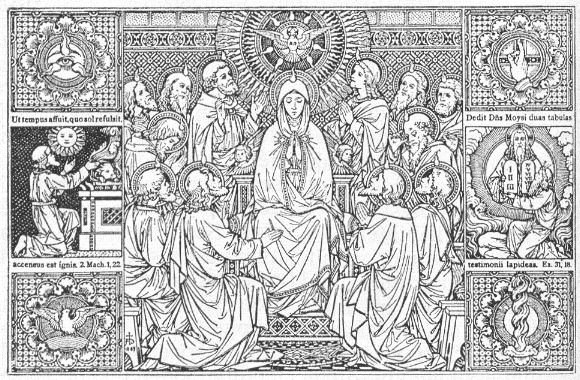
\includegraphics[width=0.95\linewidth]{Lithographie-Pfingsten-gross.jpg}};
	\end{tikzpicture}
\end{center}
\null 
\vspace*{-1.6cm}

\begin{multicols}{2}
\privdieii{}{Dominica Pentecostes}{}{Duplex I classis cum Octava privilegiata I ordinis}
\hora{In I Vesperis}

\rubric{Antiphona \black{Dum compleréntur}, cum reliquis de Laudibus. Psalmi de Dominica.}

\lectiocap{Capitulum}{Act. 2, 1-2}
\y{C}{um} compleréntur dies Pentecóstes, erant omnes discípuli páriter in eódem loco: et factus est repénte de cælo sonus, tamquam adveniéntis spíritus veheméntis, et replévit totam domum, ubi erant sedéntes.

\Rbr Spíritus Paráclitus, \red{*} Allelúja, allelúja.
\red{S}píritus.
\V Docébit vos ómnia.
\red{A}llelúja.
\red{G}lória Patri.
\red{S}píritus.

\rubric{Prima stropha Hymni sequentis dicitur flexis genibus.}

\pars{Hymnus}
\begin{hymnus}
	\y{V}{eni}, Creátor Spíritus,\\
	\hspace{1.6em} Mentes tuórum vísita,\\
Imple supérna grátia,\\
Quæ tu creásti péctora.

\red{Q}ui Paráclitus díceris,\\
Donum Dei Altíssimi,\\
Fons vivus, ignis, cáritas,\\
Et spiritális únctio.

\red{T}u septifórmis múnere,\\
Dextræ Dei tu dígitus,\\
Tu rite promíssum Patris,\\
Sermóne ditans gúttura.

\red{A}ccénde lumen sénsibus:\\
Infúnde amórem córdibus:\\
Infírma nostri córporis\\
Virtúte firmans pérpeti.

\red{H}ostem repéllas lóngjus,\\
Pacémque dones prótinus:\\
Ductóre sic te prǽvio\\
Vitémus omne nóxium.

\red{P}er te sciámus da Patrem,\\
Noscámus atque Fílium,\\
Te utriúsque Spíritum\\
Credámus omni témpore.

\red{G}lória Patri Dómino,\\
Natóque, qui a mórtuis\\
Surréxit, ac Paráclito,\\
In sæculórum sǽcula.
\red{A}men.
\end{hymnus}

\rubric{Sic terminantur omnes Hymni usque ad Nonam Sabbati sequentis inclusive.}

\V Repléti sunt omnes Spíritu Sancto, allelúja.
\R Et cœpérunt loqui, allelúja.

\M Non vos relínquam \f órphanos, allelúja: vado et vénio ad vos, allelúja: et gaudébit cor vestrum, allelúja.

\pars{Oratio}
\y{D}eus, qui hodiérna die corda fidélium Sancti Spíritus illustratióne docuísti: da nobis in eódem Spíritu recta sápere; et de ejus semper consolatióne gaudére. Per Dóminum … in unitáte ejúsdem Spíritus Sancti.

\hora{Ad Laudes}
\etper

\Av{1} Cum compleréntur \f dies Pentecóstes, erant omnes páriter in eódem loco, allelúja.
\Dominusregnavit

\Av{2} Spíritus Dómini \f replévit orbem terrárum, allelúja.

\Av{3} Repléti sunt omnes \f Spíritu Sancto, et cœpérunt loqui, allelúja, allelúja.

\Av{4} Fontes, et ómnia \f quæ movéntur in aquis, hymnum dícite Deo, allelúja.

\Av{5} Loquebántur \f váriis linguis Apóstoli magnália Dei, allelúja, allelúja, allelúja.

\lectiocap{Capitulum}{Act. 2, 1-2}
\y{C}{um} compleréntur dies Pentecóstes, erant omnes discípuli páriter in eódem loco: et factus est repénte de cælo sonus, tamquam adveniéntis spíritus veheméntis, et replévit totam domum, ubi erant sedéntes.

\Rbr Spíritus Dómini replévit orbem terrárum, \red{*} Allelúja, allelúja.
\red{S}píritus.
\V Et hoc quod cóntinet ómnia, sciéntiam habet vocis.
\red{A}llelúja.
\red{G}lória Patri.
\red{S}píritus.

\pars{Hymnus}
\begin{hymnus}
	\y{B}eáta nobis gáudia\\
	\hspace{1.6em} Anni redúxit órbita,\\
Cum Spíritus Paráclitus\\
Effúlsit in discípulos.

\red{I}gnis vibránte lúmine\\
Linguæ figúram détulit,\\
Verbis ut essent próflui,\\
Et caritáte férvidi.

\red{L}inguis loquúntur ómnium;\\
Turbæ pavent Gentílium,\\
Musto madére députant\\
Quos Spíritus repléverat.

\red{P}atráta sunt hæc mýstice,\\
Paschæ perácto témpore,\\
Sacro diérum número,\\
Quo lege fit remíssio.

\red{T}e nunc, Deus piíssime,\\
Vultu precámur cérnuo:\\
Illápsa nobis cǽlitus\\
Largíre dona Spíritus.

\red{D}udum sacráta péctora\\
Tua replésti grátia:\\
Dimítte nostra crímina,\\
Et da quiéta témpora.

\red{G}lória Patri Dómino,\\
Natóque, qui a mórtuis\\
Surréxit, ac Paráclito,\\
In sæculórum sǽcula.
\red{A}men.
\end{hymnus}

\V Repléti sunt omnes Spíritu Sancto, allelúja.
\R Et cœpérunt loqui, allelúja.

\B Accípite \f Spíritum Sanctum: quorum remiséritis peccáta, remittúntur eis, allelúja.

{\setstretch{0.995}
\pars{Oratio}
\y{D}eus, qui hodiérna die corda fidélium Sancti Spíritus illustratióne docuísti: da nobis in eódem Spíritu recta sápere; et de ejus semper consolatióne gaudére. Per Dóminum … in unitáte ejúsdem Spíritus Sancti.

\hora{Ad Tertiam}

\rubric{Hymnus \black{Veni Creátor}, ut supra ad Vesperas. Qui dicitur ad Tertiam per totam Octavam, loco Hymni \black{Nunc Sancte.}}

\rubric{Capitulum ut supra ad Laudes.}

\V Spíritus Dómini replévit orbem terrárum, allelúja.
\R Et hoc quod cóntinet ómnia, sciéntiam habet vocis, allelúja.

\hora{Ad Sextam}
\lectiocap{Capitulum}{Act. 2, 6}
\y{F}{acta} autem hac voce, convénit multitúdo, et mente confúsa est, quóniam audiébat unusquísque lingua sua illos loquéntes.

\V Spíritus Paráclitus, allelúja.
\R Docébit vos ómnia, allelúja.

\hora{Ad Nonam}
\lectiocap{Capitulum}{Act. 2, 11}
\y{J}{udǽi} quoque et Prosélyti, Cretes et Arabes: audívimus eos loquéntes nostris linguis magnália Dei.

\V Repléti sunt omnes Spíritu Sancto, allelúja.
\R Et cœpérunt loqui, allelúja.

\hora{In II Vesperis}

\rubric{Omnia ut in I Vesperis præter sequentia.}

\V Loquebántur váriis linguis Apóstoli, allelúja.
\R Magnália Dei, allelúja.

\M Hódie \f compléti sunt dies Pentecóstes, allelúja: hódie Spíritus Sanctus in igne discípulis appáruit, et tríbuit eis charísmatum dona: misit eos in univérsum mundum prædicáre, et testificári: Qui credíderit et baptizátus fúerit, salvus erit, allelúja.

\dietii{Feria II}{Infra Octavam Pentecostes}{}{Duplex I classis}
\chead{\trim{}{Feria II Infra Octavam Pentecostes}}

\B Sic Deus \f diléxit mundum, ut Fílium suum unigénitum daret: ut omnis, qui credit in ipsum, non péreat, sed hábeat vitam ætérnam, allelúja.

\pars{Oratio}
\y{D}{eus}, qui Apóstolis tuis Sanctum dedísti Spíritum: concéde plebi tuæ piæ petitiónis efféctum; ut, quibus dedísti fidem, largiáris et pacem. Per Dóminum … in unitáte ejúsdem Spíritus.

\M Si quis díligit me, \f sermónem meum servábit; et Pater meus díliget eum, et ad eum veniémus, et mansiónem apud eum faciémus, allelúja.

}
\end{multicols}


\pagebreak
\thispagestyle{empty}
\null
\vspace*{-2cm}
\begin{center}
	\begin{tikzpicture}[remember picture]
		\node at (0,0) {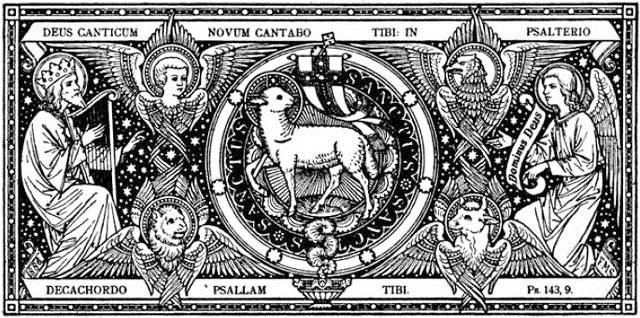
\includegraphics[width=0.95\linewidth]{Lithographie-Lamm-Evangelisten.jpg}};
	\end{tikzpicture}
\end{center}
\null 
\vspace*{-.6cm}

{\centering
	\large{EXCERPTUM EX}

	\vspace{.3em}

	\red{\Huge{PSALTERIUM}}

	\vspace{.1em}

	\normalsize{SECUNDUM REGULAM}

	\vspace{.3em}

	\red{\large{SS. PATRIS NOSTRI BENEDICTI}}

	\vspace{-.5em}

	\null
}

\begin{multicols}{2}

	{\setstretch{0.98}

\dieii{}{Sabbato}{}{}
\hora{Ad Primam}

\begin{psalmus}
\pars{Divisio Psalmi 17}
\Y{C}{um} sancto sanctus eris, * et cum viro innocénte ínnocens eris:

Et cum elécto eléctus eris: * et cum pervérso pervertéris.

Quóniam tu pópulum húmilem salvum fácies: * et óculos superbórum humiliábis.

Quóniam tu illúminas lucérnam meam, Dómine: * Deus meus, illúmina ténebras meas.

Quóniam in te erípiar a tentatióne, * et in Deo meo transgrédiar murum.

Deus meus, impollúta via ejus: \f elóquia Dómini igne examináta: * protéctor est ómnium sperántium in se.

Quóniam quis Deus præter Dóminum? * aut quis Deus præter Deum nostrum?

Deus, qui præcínxit me virtúte: * et pósuit immaculátam vjam meam.

Qui perfécit pedes meos tamquam cervórum, * et super excélsa státuens me.

Qui docet manus meas ad prǽlium: * et posuísti, ut arcum ǽreum, brácchia mea.

Et dedísti mihi protectiónem salútis tuæ: * et déxtera tua suscépit me:

Et disciplína tua corréxit me in finem: * et disciplína tua ipsa me docébit.

Dilatásti gressus meos subtus me: * et non sunt infirmáta vestígia mea:

Pérsequar inimícos meos et comprehéndam illos: * et non convértar, donec defíciant.

Confríngam illos, nec póterunt stare: * cadent subtus pedes meos.

Et præcinxísti me virtúte ad bellum: * et supplantásti insurgéntes in me subtus me.

Et inimícos meos dedísti mihi dorsum, * et odiéntes me disperdidísti.

Clamavérunt, nec erat qui salvos fáceret ad Dóminum: * nec exaudívit eos.

Et commínuam illos, ut púlverem ante fáciem venti: * ut lutum plateárum delébo eos.

Erípies me de contradictiónibus pópuli: * constítues me in caput géntium.

Pópulus quem non cognóvi servívit mihi: * in audítu auris obedívit mihi.

Fílii aliéni mentíti sunt mihi, \f fílii aliéni inveteráti sunt, * et claudicavérunt a sémitis suis.

Vivit Dóminus, et benedíctus Deus meus: * et exaltétur Deus salútis meæ.

Deus, qui das vindíctas mihi, et subdis pópulos sub me: * liberátor meus de inimícis meis iracúndis.

Et ab insurgéntibus in me exaltábis me: * a viro iníquo erípies me.

Proptérea confitébor tibi in natiónibus, Dómine: * et nómini tuo psalmum dicam.

Magníficans salútes Regis ejus, \f et fáciens misericórdiam Christo suo David: * et sémini ejus usque in sǽculum.

\end{psalmus}


\begin{psalmus}
    \pars{Psalmus 18}
    
    \y{C}{æli} enárrant glóriam Dei: * et ópera mánuum ejus annúntiat firmaméntum.
    
    Dies diéi erúctat verbum, * et nox nocti índicat sciéntiam.
    
    Non sunt loquélæ, neque sermónes, * quorum non audiántur voces eórum.
    
    In omnem terram exívit sonus eórum: * et in fines orbis terræ verba eórum.
    
    In sole pósuit tabernáculum suum: * et ipse tamquam sponsus procédens de thálamo suo:
    
    Exsultávit ut gigas ad curréndam vjam, * a summo cælo egréssio ejus:
    
    Et occúrsus ejus usque ad summum ejus: * nec est qui se abscóndat a calóre ejus.
    
    Lex Dómini immaculáta, convértens ánimas: * testimónium Dómini fidéle, sapiéntiam præstans párvulis.
    
    Justítiæ Dómini rectæ, lætificántes corda: * præcéptum Dómini lúcidum, illúminans óculos.
    
    Timor Dómini sanctus, pérmanens in sǽculum sǽculi: * judícia Dómini vera, justificáta in semetípsa.
    
    Desiderabília super aurum et lápidem pretiósum multum: * et dulcióra super mel et favum.
    
    Étenim servus tuus custódit ea, * in custodiéndis illis retribútio multa.
    
    Delícta quis intéllegit? \f ab occúltis meis munda me: * et ab aliénis parce servo tuo.
    
    Si mei non fúerint domináti, tunc immaculátus ero: * et emundábor a delícto máximo.
    
    Et erunt ut compláceant elóquia oris mei: * et meditátio cordis mei in conspéctu tuo semper.
    
    Dómine, adjútor meus, * et redémptor meus.
    
    \end{psalmus}


\begin{psalmus}
\pars{Psalmus 19}

\y{E}{xáudiat} te Dóminus in die tribulatiónis: * prótegat te nomen Dei Jacob.

Mittat tibi auxílium de sancto: * et de Sion tueátur te.

Memor sit omnis sacrifícii tui: * et holocáustum tuum pingue fiat.

Tríbuat tibi secúndum cor tuum: * et omne consílium tuum confírmet.

Lætábimur in salutári tuo: * et in nómine Dei nostri magnificábimur.

Ímpleat Dóminus omnes petitiónes tuas: * nunc cognóvi quóniam salvum fecit Dóminus Christum suum.

Exáudiet illum de cælo sancto suo: * in potentátibus salus déxteræ ejus.

Hi in cúrribus, et hi in equis: * nos autem in nómine Dómini, Dei nostri invocábimus.

Ipsi obligáti sunt, et cecidérunt: * nos autem surréximus et erécti sumus.

Dómine, salvum fac regem: * et exáudi nos in die, qua invocavérimus te.

\end{psalmus}


\hora{Ad Tertiam}

\begin{psalmus}
\pars{Psalmus 119}

\Yii{A}{d} Dóminum cum tribulárer clamávi: * et exaudívit me.

Dómine, líbera ánimam meam a lábiis iníquis, * et a lingua dolósa.

Quid detur tibi, aut quid apponátur tibi * ad linguam dolósam?

Sagíttæ poténtis acútæ, * cum carbónibus desolatóriis.

Heu mihi, quia incolátus meus prolongátus est! \f habitávi cum habitántibus Cedar: * multum íncola fuit ánima mea.

Cum his, qui odérunt pacem, eram pacíficus: * cum loquébar illis, impugnábant me gratis.

\end{psalmus}


\begin{psalmus}
\pars{Psalmus 120}

\y{L}{evávi} óculos meos in montes, * unde véniet auxílium mihi.

Auxílium meum a Dómino, * qui fecit cælum et terram.

Non det in commotiónem pedem tuum: * neque dormítet qui custódit te.

Ecce, non dormitábit neque dórmiet, * qui custódit Israël.

Dóminus custódit te, Dóminus protéctio tua, * super manum déxteram tuam.

Per diem sol non uret te: * neque luna per noctem.

Dóminus custódit te ab omni malo: * custódiat ánimam tuam Dóminus.

Dóminus custódiat intróitum tuum, et éxitum tuum: * ex hoc nunc, et usque in sǽculum.

\end{psalmus}


\begin{psalmus}
    \pars{Psalmus 121}

    \y{L}{ætátus} sum in his, quæ dicta sunt mihi: * In domum Dómini íbimus.

    Stantes erant pedes nostri, * in átriis tuis, Jerúsalem.

    Jerúsalem, quæ ædificátur ut cívitas: * cujus participátio ejus in idípsum.

    Illuc enim ascendérunt tribus, tribus Dómini: * testimónium Israël ad confiténdum nómini Dómini.

    Quia illic sedérunt sedes in judício, * sedes super domum David.

    Rogáte quæ ad pacem sunt Jerúsalem: * et abundántia diligéntibus te:

    Fiat pax in virtúte tua: * et abundántia in túrribus tuis.

    Propter fratres meos, et próximos meos, * loquébar pacem de te:

    Propter domum Dómini, Dei nostri, * quæsívi bona tibi.

\end{psalmus}


\hora{Ad Sextam}

\begin{psalmus}
	\pars{Psalmus 122}

	\Yii{A}{d} te levávi óculos meos, * qui hábitas in cælis.

	Ecce, sicut óculi servórum * in mánibus dominórum suórum,

	Sicut óculi ancíllæ in mánibus dóminæ suæ: * ita óculi nostri ad Dóminum, Deum nostrum, donec misereátur nostri.

	Miserére nostri, Dómine, miserére nostri: * quia multum repléti sumus despectióne:

	Quia multum repléta est ánima nostra: * oppróbrium abundántibus, et despéctio supérbis.

\end{psalmus}


\begin{psalmus}
\pars{Psalmus 123}

\y{N}{isi} quia Dóminus erat in nobis, dicat nunc Israël: * nisi quia Dóminus erat in nobis,

Cum exsúrgerent hómines in nos, * forte vivos deglutíssent nos:

Cum irascerétur furor eórum in nos, * fórsitan aqua absorbuísset nos.

Torréntem pertransívit ánima nostra: * fórsitan pertransísset ánima nostra aquam intolerábilem.

Benedíctus Dóminus * qui non dedit nos in captiónem déntibus eórum.

Ánima nostra sicut passer erépta est * de láqueo venántium:

Láqueus contrítus est, * et nos liberáti sumus.

Adiutórium nostrum in nómine Dómini, * qui fecit cælum et terram.

\end{psalmus}


\begin{psalmus}
\pars{Psalmus 124}

\y{Q}{ui} confídunt in Dómino, sicut mons Sion: * non commovébitur in ætérnum, qui hábitat in Jerúsalem.

Montes in circúitu ejus: \f et Dóminus in circúitu pópuli sui, * ex hoc nunc et usque in sǽculum.

Quia non relínquet Dóminus virgam peccatórum super sortem justórum: * ut non exténdant justi ad iniquitátem manus suas.

Bénefac, Dómine, bonis, * et rectis corde.

Declinántes autem in obligatiónes addúcet Dóminus cum operántibus iniquitátem: * pax super Israël.

\end{psalmus}


\hora{Ad Nonam}

\begin{psalmus}
    \pars{Psalmus 125}
    
    \Yii{I}{n} converténdo Dóminus captivitátem Sion: * facti sumus sicut consoláti:
    
    Tunc replétum est gáudio os nostrum: * et lingua nostra exsultatióne.
    
    Tunc dicent inter gentes: * Magnificávit Dóminus fácere cum eis.
    
    Magnificávit Dóminus fácere nobíscum: * facti sumus lætántes.
    
    Convérte, Dómine, captivitátem nostram, * sicut torrens in Austro.
    
    Qui séminant in lácrimis, * in exsultatióne metent.
    
    Eúntes ibant et flebant, * mitténtes sémina sua.
    
    Veniéntes autem vénient cum exsultatióne, * portántes manípulos suos.
    
    \end{psalmus}


\begin{psalmus}
    \pars{Psalmus 126}

    \y{N}{isi} Dóminus ædificáverit domum, * in vanum laboravérunt qui ædíficant eam.

    Nisi Dóminus custodíerit civitátem, * frustra vígilat qui custódit eam.

    Vanum est vobis ante lucem súrgere: * súrgite postquam sedéritis, qui manducátis panem dolóris.

    Cum déderit diléctis suis somnum: * ecce heréditas Dómini fílii: merces, fructus ventris.

    Sicut sagíttæ in manu poténtis: * ita fílii excussórum.

    Beátus vir, qui implévit desidérium suum ex ipsis: * non confundétur cum loquétur inimícis suis in porta.

\end{psalmus}


\begin{psalmus}
\pars{Psalmus 127}

\y{B}{eáti}, omnes, qui timent Dóminum, * qui ámbulant in viis ejus.

Labóres mánuum tuárum quia manducábis: * beátus es, et bene tibi erit.

Uxor tua sicut vitis abúndans, * in latéribus domus tuæ.

Fílii tui sicut novéllæ olivárum, * in circúitu mensæ tuæ.

Ecce, sic benedicétur homo, * qui timet Dóminum.

Benedícat tibi Dóminus ex Sion: * et vídeas bona Jerúsalem ómnibus diébus vitæ tuæ.

Et vídeas fílios filiórum tuórum, * pacem super Israël.

\end{psalmus}


\die{}{Dominica}{}{}

\hora{Ad Laudes}

\begin{psalmus}
\pars{Psalmus 66}

\y{D}{eus} misereátur nostri, et benedícat nobis: * illúminet vultum suum super nos, et misereátur nostri.

Ut cognoscámus in terra vjam tuam, * in ómnibus géntibus salutáre tuum.

Confiteántur tibi pópuli, Deus: * confiteántur tibi pópuli omnes.

Læténtur et exsúltent gentes: \f quóniam iúdicas pópulos in æquitáte, * et gentes in terra dírigis.

Confiteántur tibi pópuli, Deus, \f confiteántur tibi pópuli omnes: * terra dedit fructum suum.

Benedícat nos Deus, Deus noster, benedícat nos Deus: * et métuant eum omnes fines terræ.
        
\end{psalmus}


\begin{psalmus}
\pars{Psalmus 92}

\Y{D}{óminus} regnávit, decórem indútus est: * indútus est Dóminus fortitúdinem, et præcínxit se.

Étenim firmávit orbem terræ, * qui non commovébitur.

Paráta sedes tua ex tunc: * a sǽculo tu es.

Elevavérunt flúmina, Dómine: * elevavérunt flúmina vocem suam.

Elevavérunt flúmina fluctus suos, * a vócibus aquárum multárum.

Mirábiles elatiónes maris: * mirábilis in altis Dóminus.

Testimónia tua credibília facta sunt nimis: * domum tuam decet sanctitúdo, Dómine, in longitúdinem diérum. 

\end{psalmus}


\begin{psalmus}
\pars{Psalmus 99}

\y{J}{ubiláte} Deo, omnis terra: * servíte Dómino in lætítia.

Introíte in conspéctu ejus, * in exsultatióne.

Scitóte quóniam Dóminus ipse est Deus: * ipse fecit nos, et non ipsi nos.

Pópulus ejus, et oves páscuæ ejus. \f Introíte portas ejus in confessióne, * átria ejus in hymnis: confitémini illi.

Laudáte nomen ejus: quóniam suávis est Dóminus, \f in ætérnum misericórdia ejus, * et usque in generatiónem et generatiónem véritas ejus.

\end{psalmus}


\begin{psalmus}
\pars{Psalmus 62}

\y{D}{eus}, Deus meus, * ad te de luce vígilo.

Sitívit in te ánima mea, * quam multiplíciter tibi caro mea.

In terra desérta, et ínvia, et inaquósa: \f sic in sancto appárui tibi, * ut vidérem virtútem tuam, et glóriam tuam.

Quóniam mélior est misericórdia tua super vitas: * lábia mea laudábunt te.

Sic benedícam te in vita mea: * et in nómine tuo levábo manus meas.

Sicut ádipe et pinguédine repleátur ánima mea: * et lábiis exsultatiónis laudábit os meum.

Si memor fui tui super stratum meum, \f in matutínis meditábor in te: * quia fuísti adiútor meus.

Et in velaménto alárum tuárum exsultábo, \f adhǽsit ánima mea post te: * me suscépit déxtera tua.

Ipsi vero in vanum quæsiérunt ánimam meam, \f introíbunt in inferióra terræ: * tradéntur in manus gládii, partes vúlpium erunt.

Rex vero lætábitur in Deo, \f laudabúntur omnes qui jurant in eo: * quia obstrúctum est os loquéntium iníqua.

\end{psalmus}


\begin{psalmus}
\lectiocap{Canticum trium puerorum}{Dan. 3, 57-88 et 56}

\y{B}{enedícite}, ómnia ópera Dómini, Dómino: * laudáte et superexaltáte eum in sǽcula.

Benedícite, Ángeli Dómini, Dómino: * benedícite, cæli, Dómino.

Benedícite, aquæ omnes, quæ super cælos sunt, Dómino: * benedícite, omnes virtútes Dómini, Dómino.

Benedícite, sol et luna, Dómino: * benedícite, stellæ cæli, Dómino.

Benedícite, omnis imber et ros, Dómino: * benedícite, omnes spíritus Dei, Dómino.

Benedícite, ignis et æstus, Dómino: * benedícite, frigus et æstus, Dómino.

Benedícite, rores et pruína, Dómino: * benedícite, gelu et frigus, Dómino.

Benedícite, glácies et nives, Dómino: * benedícite, noctes et dies, Dómino.

Benedícite, lux et ténebræ, Dómino: * benedícite, fúlgura et nubes, Dómino.

Benedícat terra Dóminum: * laudet et superexáltet eum in sǽcula.

Benedícite, montes et colles, Dómino: * benedícite, univérsa germinántia in terra, Dómino.

Benedícite, fontes, Dómino: * benedícite, mária et flúmina, Dómino.

Benedícite, cete, et ómnia, quæ movéntur in aquis, Dómino: * benedícite, omnes vólucres cæli, Dómino.

Benedícite, omnes béstiæ et pécora, Dómino: * benedícite, fílii hóminum, Dómino.

Benedícat Israël Dóminum: * laudet et superexáltet eum in sǽcula.

Benedícite, sacerdótes Dómini, Dómino: * benedícite, servi Dómini, Dómino.

Benedícite, spíritus, et ánimæ justórum, Dómino: * benedícite, sancti, et húmiles corde, Dómino.

Benedícite, Ananía, Azaría, Mísaël, Dómino: * laudáte et superexaltáte eum in sǽcula.

Benedicámus Patrem et Fílium cum Sancto Spíritu: * laudémus et superexaltémus eum in sǽcula.

Benedíctus es, Dómine, in firmaménto cæli: * et laudábilis, et gloriósus, et superexaltátus in sǽcula.

\rubric{Hic non dicitur \black{Glória Patri} neque \black{Amen.}}

\end{psalmus}


\begin{psalmus}
\pars{Psalmus 148}

\y{L}{audáte} Dóminum de cælis: * laudáte eum in excélsis.

Laudáte eum, omnes Ángeli ejus: * laudáte eum, omnes virtútes ejus.

Laudáte eum, sol et luna: * laudáte eum, omnes stellæ et lumen.

Laudáte eum, cæli cælórum: * et aquæ omnes, quæ super cælos sunt, laudent nomen Dómini.

Quia ipse dixit, et facta sunt: * ipse mandávit, et creáta sunt.

Státuit ea in ætérnum, et in sǽculum sǽculi: * præcéptum pósuit, et non præteríbit.

Laudáte Dóminum de terra, * dracónes, et omnes abýssi.

Ignis, grando, nix, glácies, spíritus procellárum: * quæ fáciunt verbum ejus:

Montes, et omnes colles: * ligna fructífera, et omnes cedri.

Béstiæ, et univérsa pécora: * serpéntes, et vólucres pennátæ:

Reges terræ, et omnes pópuli: * príncipes, et omnes iúdices terræ.

Iúvenes, et vírgines: \f senes cum iunióribus laudent nomen Dómini: * quia exaltátum est nomen ejus solíus.

Conféssio ejus super cælum et terram: * et exaltávit cornu pópuli sui.

Hymnus ómnibus sanctis ejus: * fíliis Israël, pópulo appropinquánti sibi.

\rubric{Hic non dicitur \black{Glória Patri.}}

\pars{Psalmus 149}

\y{C}{antáte} Dómino cánticum novum: * laus ejus in ecclésia sanctórum.

Lætétur Israël in eo, qui fecit eum: * et fílii Sion exsúltent in rege suo.

Laudent nomen ejus in choro: * in týmpano, et psaltério psallant ei:

Quia beneplácitum est Dómino in pópulo suo: * et exaltábit mansuétos in salútem.

Exsultábunt sancti in glória: * lætabúntur in cubílibus suis.

Exaltatiónes Dei in gútture eórum: * et gládii ancípites in mánibus eórum.

Ad faciéndam vindíctam in natiónibus: * increpatiónes in pópulis.

Ad alligándos reges eórum in compédibus: * et nóbiles eórum in mánicis férreis.

Ut fáciant in eis judícium conscríptum: * glória hæc est ómnibus sanctis ejus.

\rubric{Hic non dicitur \black{Glória Patri.}}

\pars{Psalmus 150}

\y{L}{audáte} Dóminum in sanctis ejus: * laudáte eum in firmaménto virtútis ejus.

Laudáte eum in virtútibus ejus: * laudáte eum secúndum multitúdinem magnitúdinis ejus.

Laudáte eum in sono tubæ: * laudáte eum in psaltério, et cíthara.

Laudáte eum in týmpano, et choro: * laudáte eum in chordis, et órgano.

Laudáte eum in cýmbalis benesonántibus: \f laudáte eum in cýmbalis jubilatiónis: * omnis spíritus laudet Dóminum.

Glória Patri.

\end{psalmus}


\hora{Ad Primam}

\begin{psalmus}
\pars{Psalmus 118, 1}

\Y{B}{eáti} \hspace{.5em} immaculáti \hspace{.5em} in \hspace{.5em} via: * qui ámbulant in lege Dómini.

Beáti, qui scrutántur testimónia ejus: * in toto corde exquírunt eum.

Non enim qui operántur iniquitátem, * in viis ejus ambulavérunt.

Tu mandásti * mandáta tua custodíri nimis.

Útinam dirigántur viæ meæ, * ad custodiéndas justificatiónes tuas!

Tunc non confúndar, * cum perspéxero in ómnibus mandátis tuis.

Confitébor tibi in directióne cordis: * in eo quod dídici judícia justítiæ tuæ.

Iustificatiónes tuas custódiam: * non me derelínquas usquequáque.

\end{psalmus}


\begin{psalmus}
\pars{Psalmus 118, 2}

\y{I}{n} quo córrigit adolescéntior vjam suam? * In custodiéndo sermónes tuos.

In toto corde meo exquisívi te: * ne repéllas me a mandátis tuis.

In corde meo abscóndi elóquia tua: * ut non peccem tibi.

Benedíctus es, Dómine: * doce me justificatiónes tuas.

In lábiis meis, * pronuntiávi ómnia judícia oris tui.

In via testimoniórum tuórum delectátus sum, * sicut in ómnibus divítiis.

In mandátis tuis exercébor: * et considerábo vias tuas.

In justificatiónibus tuis meditábor: * non oblivíscar sermónes tuos.

\end{psalmus}


\begin{psalmus}
\pars{Psalmus 118, 3}

\y{R}{etríbue} servo tuo, vivífica me: * et custódiam sermónes tuos:

Revéla óculos meos: * et considerábo mirabília de lege tua.

Íncola ego sum in terra: * non abscóndas a me mandáta tua.

Concupívit ánima mea desideráre justificatiónes tuas, * in omni témpore.

Increpásti supérbos: * maledícti qui declínant a mandátis tuis.

Aufer a me oppróbrium, et contémptum: * quia testimónia tua exquisívi.

Étenim sedérunt príncipes, et advérsum me loquebántur: * servus autem tuus exercebátur in justificatiónibus tuis.

Nam et testimónia tua meditátio mea est: * et consílium meum justificatiónes tuæ.

\end{psalmus}


\begin{psalmus}
\pars{Psalmus 118, 4}

\y{A}{dhǽsit} paviménto ánima mea: * vivífica me secúndum verbum tuum.

Vias meas enuntiávi, et exaudísti me: * doce me justificatiónes tuas.

Vjam justificatiónum tuárum ínstrue me: * et exercébor in mirabílibus tuis.

Dormitávit ánima mea præ tǽdio: * confírma me in verbis tuis.

Vjam iniquitátis ámove a me: * et de lege tua miserére mei.

Vjam veritátis elégi: * judícia tua non sum oblítus.

Adhǽsi testimóniis tuis, Dómine: * noli me confúndere.

Vjam mandatórum tuórum cucúrri, * cum dilatásti cor meum.

\end{psalmus}


\hora{Ad Tertiam}

\vspace{-.5em}

\begin{psalmus}
\pars{Psalmus 118, 5}

\Yii{L}{egem} pone mihi, Dómine, vjam justificatiónum tuárum: * et exquíram eam semper.

Da mihi intelléctum, et scrutábor legem tuam: * et custódiam illam in toto corde meo.

Deduc me in sémitam mandatórum tuórum: * quia ipsam vólui.

Inclína cor meum in testimónia tua: * et non in avarítiam.

Avérte óculos meos ne vídeant vanitátem: * in via tua vivífica me.

Státue servo tuo elóquium tuum, * in timóre tuo.

Ámputa oppróbrium meum quod suspicátus sum: * quia judícia tua jucúnda.

Ecce, concupívi mandáta tua: * in æquitáte tua vivífica me.

\end{psalmus}


\begin{psalmus}
\pars{Psalmus 118, 6}

\y{E}{t} véniat super me misericórdia tua, Dómine: * salutáre tuum secúndum elóquium tuum.

Et respondébo exprobrántibus mihi verbum: * quia sperávi in sermónibus tuis.

Et ne áuferas de ore meo verbum veritátis usquequáque: * quia in judíciis tuis supersperávi.

Et custódiam legem tuam semper: * in sǽculum et in sǽculum sǽculi.

Et ambulábam in latitúdine: * quia mandáta tua exquisívi.

Et loquébar in testimóniis tuis in conspéctu regum: * et non confundébar.

Et meditábar in mandátis tuis, * quæ diléxi.

Et levávi manus meas ad mandáta tua, quæ diléxi: * et exercébar in justificatiónibus tuis.

\end{psalmus}


\begin{psalmus}
\pars{Psalmus 118, 7}

\y{M}{emor} esto verbi tui servo tuo, * in quo mihi spem dedísti.

Hæc me consoláta est in humilitáte mea: * quia elóquium tuum vivificávit me.

Supérbi iníque agébant usquequáque: * a lege autem tua non declinávi.

Memor fui judiciórum tuórum a sǽculo, Dómine: * et consolátus sum.

Deféctio ténuit me, * pro peccatóribus derelinquéntibus legem tuam.

Cantábiles mihi erant justificatiónes tuæ, * in loco peregrinatiónis meæ.

Memor fui nocte nóminis tui, Dómine: * et custodívi legem tuam.

Hæc facta est mihi: * quia justificatiónes tuas exquisívi.

\end{psalmus}


\vspace{-.1em}

\hora{Ad Sextam}

\vspace{-.5em}

\begin{psalmus}
\pars{Psalmus 118, 8}

\Yii{P}{órtio} mea, Dómine, * dixi custodíre legem tuam.

Deprecátus sum fáciem tuam in toto corde meo: * miserére mei secúndum elóquium tuum.

Cogitávi vias meas: * et convérti pedes meos in testimónia tua.

Parátus sum, et non sum turbátus: * ut custódiam mandáta tua.

Funes peccatórum circumpléxi sunt me: * et legem tuam non sum oblítus.

Média nocte surgébam ad confiténdum tibi, * super judícia justificatiónis tuæ.

Párticeps ego sum ómnium timéntium te: * et custodiéntium mandáta tua.

Misericórdia tua, Dómine, plena est terra: * justificatiónes tuas doce me.

\end{psalmus}


\vspace{-.1em}

\begin{psalmus}
\pars{Psalmus 118, 9}

\y{B}{onitátem} fecísti cum servo tuo, Dómine, * secúndum verbum tuum.

Bonitátem, et disciplínam, et sciéntiam doce me: * quia mandátis tuis crédidi.

Priúsquam humiliárer ego delíqui: * proptérea elóquium tuum custodívi.

Bonus es tu: * et in bonitáte tua doce me justificatiónes tuas.

Multiplicáta est super me iníquitas superbórum: * ego autem in toto corde meo scrutábor mandáta tua.

Coagulátum est sicut lac cor eórum: * ego vero legem tuam meditátus sum.

Bonum mihi quia humiliásti me: * ut discam justificatiónes tuas.

Bonum mihi lex oris tui, * super míllia auri et argénti.

\end{psalmus}


\columnbreak

\begin{psalmus}
\pars{Psalmus 118, 10}

\y{M}{anus} tuæ fecérunt me, et plasmavérunt me: * da mihi intelléctum, et discam mandáta tua.

Qui timent te vidébunt me, et lætabúntur: * quia in verba tua supersperávi.

Cognóvi, Dómine, quia ǽquitas judícia tua: * et in veritáte tua humiliásti me.

Fiat misericórdia tua ut consolétur me, * secúndum elóquium tuum servo tuo.

Véniant mihi miseratiónes tuæ, et vivam: * quia lex tua meditátio mea est.

Confundántur supérbi, quia iniúste iniquitátem fecérunt in me: * ego autem exercébor in mandátis tuis.

Convertántur mihi timéntes te: * et qui novérunt testimónia tua.

Fiat cor meum immaculátum in justificatiónibus tuis, * ut non confúndar.

\end{psalmus}


\ornamentvii
\columnbreak

\hora{Ad Nonam}

\begin{psalmus}
\pars{Psalmus 118, 11}

\Yii{D}{efécit} in salutáre tuum ánima mea: * et in verbum tuum supersperávi.

Defecérunt óculi mei in elóquium tuum, * dicéntes: Quando consoláberis me?

Quia factus sum sicut uter in pruína: * justificatiónes tuas non sum oblítus.

Quot sunt dies servi tui? * quando fácies de persequéntibus me judícium?

Narravérunt mihi iníqui fabulatiónes: * sed non ut lex tua.

Ómnia mandáta tua véritas: * iníque persecúti sunt me, ádjuva me.

Paulo minus consummavérunt me in terra: * ego autem non derelíqui mandáta tua.

Secúndum misericórdiam tuam vivífica me: * et custódiam testimónia oris tui.

\end{psalmus}


\begin{psalmus}
\pars{Psalmus 118, 12}

\y{I}{n} ætérnum, Dómine, * verbum tuum pérmanet in cælo.

In generatiónem et generatiónem véritas tua: * fundásti terram, et pérmanet.

Ordinatióne tua persevérat dies: * quóniam ómnia sérviunt tibi.

Nisi quod lex tua meditátio mea est: * tunc forte periíssem in humilitáte mea.

In ætérnum non oblivíscar justificatiónes tuas: * quia in ipsis vivificásti me.

Tuus sum ego, salvum me fac: * quóniam justificatiónes tuas exquisívi.

Me exspectavérunt peccatóres ut pérderent me: * testimónia tua intelléxi.

Omnis consummatiónis vidi finem: * latum mandátum tuum nimis.

\end{psalmus}


\begin{psalmus}
\pars{Psalmus 118, 13}

\y{Q}{uómodo} diléxi legem tuam, Dómine? * tota die meditátio mea est.

Super inimícos meos prudéntem me fecísti mandáto tuo: * quia in ætérnum mihi est.

Super omnes docéntes me intelléxi: * quia testimónia tua meditátio mea est.

Super senes intelléxi: * quia mandáta tua quæsívi.

Ab omni via mala prohíbui pedes meos: * ut custódiam verba tua.

A judíciis tuis non declinávi: * quia tu legem posuísti mihi.

Quam dúlcia fáucibus meis elóquia tua, * super mel ori meo!

A mandátis tuis intelléxi: * proptérea odívi omnem vjam iniquitátis.

\end{psalmus}


\hora{Ad Vesperas}

\begin{psalmus}
\pars{Psalmus 109}

\Y{D}{ixit} \hspace{.5em} Dóminus \hspace{.5em} Dómino meo: \hspace{.5em} * \hspace{.5em} Sede \hspace{.5em} a \hspace{.5em} dextris meis:

Donec ponam inimícos tuos, * scabéllum pedum tuórum.

Virgam virtútis tuæ emíttet Dóminus ex Sion: * domináre in médio inimicórum tuórum.

Tecum princípium in die virtútis tuæ in splendóribus sanctórum: * ex útero ante lucíferum génui te.

Jurávit Dóminus, et non pœnitébit eum: * Tu es sacérdos in ætérnum secúndum órdinem Melchísedech.

Dóminus a dextris tuis, * confrégit in die iræ suæ reges.

Judicábit in natiónibus, implébit ruínas: * conquassábit cápita in terra multórum.

De torrénte in via bibet: * proptérea exaltábit caput.

\end{psalmus}


\begin{psalmus}
    \pars{Psalmus 110}

    \y{C}{onfitébor} tibi, Dómine, in toto corde meo: * in consílio justórum, et congregatióne.

    Magna ópera Dómini: * exquisíta in omnes voluntátes ejus.

    Conféssio et magnificéntia opus ejus: * et justítia ejus manet in sǽculum sǽculi.

    Memóriam fecit mirabílium suórum, \f miséricors et miserátor Dóminus: * escam dedit timéntibus se.

    Memor erit in sǽculum testaménti sui: * virtútem óperum suórum annuntiábit pópulo suo:

    Ut det illis hereditátem géntium: * ópera mánuum ejus véritas, et judícium.

    Fidélia ómnia mandáta ejus: \f confirmáta in sǽculum sǽculi, * facta in veritáte et æquitáte.

    Redemptiónem misit pópulo suo: * mandávit in ætérnum testaméntum suum.

    Sanctum, et terríbile nomen ejus: * inítium sapiéntiæ timor Dómini.

    Intelléctus bonus ómnibus faciéntibus eum: * laudátio ejus manet in sǽculum sǽculi.

\end{psalmus}


\begin{psalmus}
    \pars{Psalmus 111}

    \y{B}{eátus} vir, qui timet Dóminum: * in mandátis ejus volet nimis.

    Potens in terra erit semen ejus * generátio rectórum benedicétur.

    Glória, et divítiæ in domo ejus * et justítia ejus manet in sǽculum sǽculi.

    Exórtum est in ténebris lumen rectis * miséricors, et miserátor, et justus.

    Jucúndus homo qui miserétur et cómmodat, \f dispónet sermónes suos in judício: * quia in ætérnum non commovébitur.

    In memória ætérna erit justus * ab auditióne mala non timébit.

    Parátum cor ejus speráre in Dómino, \f confirmátum est cor ejus * non commovébitur donec despíciat inimícos suos.

    Dispérsit, dedit paupéribus: \f justítia ejus manet in sǽculum sǽculi, * cornu ejus exaltábitur in glória.

    Peccátor vidébit, et irascétur, \f déntibus suis fremet et tabéscet * desidérium peccatórum períbit.

\end{psalmus}


\begin{psalmus}
    \pars{Psalmus 112}

    \y{L}{audáte}, púeri, Dóminum: * laudáte nomen Dómini.

    Sit nomen Dómini benedíctum, * ex hoc nunc, et usque in sǽculum.

    A solis ortu usque ad occásum, * laudábile nomen Dómini.

    Excélsus super omnes gentes Dóminus, * et super cælos glória ejus.

    Quis sicut Dóminus, Deus noster, qui in altis hábitat, * et humília réspicit in cælo et in terra?

    Súscitans a terra ínopem, * et de stércore érigens páuperem:

    Ut cóllocet eum cum princípibus, * cum princípibus pópuli sui.

    Qui habitáre facit stérilem in domo, * matrem filiórum lætántem.

\end{psalmus}


\die{}{Feria II}{}{}

\hora{Ad Primam}

\begin{psalmus}
    \pars{Psalmus 1}

    \Y{B}{eátus} vir, qui non ábiit in consílio impiórum, \f et in via peccatórum non stetit, * et in cáthedra pestiléntiæ non sedit:

    Sed in lege Dómini volúntas ejus, * et in lege ejus meditábitur die ac nocte.

    Et erit tamquam lignum, quod plantátum est secus decúrsus aquárum, * quod fructum suum dabit in témpore suo:

    Et fólium ejus non défluet: * et ómnia quæcúmque fáciet, prosperabúntur.

    Non sic ímpii, non sic: * sed tamquam pulvis, quem proícit ventus a fácie terræ.

    Ídeo non resúrgent ímpii in judício: * neque peccatóres in concílio justórum.

    Quóniam novit Dóminus vjam justórum: * et iter impiórum períbit.

\end{psalmus}


\begin{psalmus}
    \pars{Psalmus 2}

    \y{Q}{uare} fremuérunt gentes: * et pópuli meditáti sunt inánia?

		Astitérunt reges terræ, et príncipes convenérunt in unum * advérsus Dóminum, et advérsus Christum ejus.

    Dirumpámus víncula eórum: * et proiciámus a nobis jugum ipsórum.

    Qui hábitat in cælis, irridébit eos: * et Dóminus subsannábit eos.

    Tunc loquétur ad eos in ira sua, * et in furóre suo conturbábit eos.

    Ego autem constitútus sum Rex ab eo super Sion montem sanctum ejus, * prǽdicans præcéptum ejus.

    Dóminus dixit ad me: * Fílius meus es tu, ego hódie génui te.

    Póstula a me, et dabo tibi gentes hereditátem tuam, * et possessiónem tuam términos terræ.

    Reges eos in virga férrea, * et tamquam vas fíguli confrínges eos.

    Et nunc, reges, intellégite: * erudímini, qui judicátis terram.

    Servíte Dómino in timóre: * et exsultáte ei cum tremóre.

    Apprehéndite disciplínam, nequándo irascátur Dóminus, * et pereátis de via justa.

\end{psalmus}


\begin{psalmus}
\pars{Psalmus 6}

\y{D}{ómine}, ne in furóre tuo árguas me, * neque in ira tua corrípias me.

Miserére mei, Dómine, quóniam infírmus sum: * sana me, Dómine, quóniam conturbáta sunt ossa mea.

Et ánima mea turbáta est valde: * sed tu, Dómine, úsquequo?

Convértere, Dómine, et éripe ánimam meam: * salvum me fac propter misericórdiam tuam.

Quóniam non est in morte qui memor sit tui: * in inférno autem quis confitébitur tibi?

Laborávi in gémitu meo, \f lavábo per síngulas noctes lectum meum: * lácrimis meis stratum meum rigábo.

Turbátus est a furóre óculus meus: * inveterávi inter omnes inimícos meos.

Discédite a me, omnes, qui operámini iniquitátem: * quóniam exaudívit Dóminus vocem fletus mei.

Exaudívit Dóminus deprecatiónem meam, * Dóminus oratiónem meam suscépit.

Erubéscant, et conturbéntur veheménter omnes inimíci mei: * convertántur et erubéscant valde velóciter.

\end{psalmus}


\ornamentviii

\columnbreak
\hora{Ad Tertiam}

\begin{psalmus}
\pars{Psalmus 118, 14}

\Yii{L}{ucérna} pédibus meis verbum tuum, * et lumen sémitis meis.

Iurávi, et státui * custodíre judícia justítiæ tuæ.

Humiliátus sum usquequáque, Dómine: * vivífica me secúndum verbum tuum.

Voluntária oris mei beneplácita fac, Dómine: * et judícia tua doce me.

Ánima mea in mánibus meis semper: * et legem tuam non sum oblítus.

Posuérunt peccatóres láqueum mihi: * et de mandátis tuis non errávi.

Hereditáte acquisívi testimónia tua in ætérnum: * quia exsultátio cordis mei sunt.

Inclinávi cor meum ad faciéndas justificatiónes tuas in ætérnum, * propter retributiónem.

\end{psalmus}


\begin{psalmus}
\pars{Psalmus 118, 15}

\y{I}{níquos} ódio hábui: * et legem tuam diléxi.

Adiútor et suscéptor meus es tu: * et in verbum tuum supersperávi.

Declináte a me, malígni: * et scrutábor mandáta Dei mei.

\textsc{Súscipe me secúndum elóquium tuum, et vivam: * et non confúndas me ab exspectatióne mea.}

Ádjuva me, et salvus ero: * et meditábor in justificatiónibus tuis semper.

Sprevísti omnes discedéntes a judíciis tuis: * quia iniústa cogitátio eórum.

Prævaricántes reputávi omnes peccatóres terræ: * ídeo diléxi testimónia tua.

Confíge timóre tuo carnes meas: * a judíciis enim tuis tímui.

\end{psalmus}


\begin{psalmus}
\pars{Psalmus 118, 16}

\y{F}{eci} judícium et justítiam: * non tradas me calumniántibus me.

Súscipe servum tuum in bonum: * non calumniéntur me supérbi.

Óculi mei defecérunt in salutáre tuum: * et in elóquium justítiæ tuæ.

Fac cum servo tuo secúndum misericórdiam tuam: * et justificatiónes tuas doce me.

Servus tuus sum ego: * da mihi intelléctum, ut scjam testimónia tua.

Tempus faciéndi, Dómine: * dissipavérunt legem tuam.

Ídeo diléxi mandáta tua, * super aurum et topázion.

Proptérea ad ómnia mandáta tua dirigébar: * omnem vjam iníquam ódio hábui.

\end{psalmus}


\hora{Ad Sextam}

\begin{psalmus}
\pars{Psalmus 118, 17}

\Yii{M}{irabília} testimónia tua: * ídeo scrutáta est ea ánima mea.

Declarátio sermónum tuórum illúminat: * et intelléctum dat párvulis.

Os meum apérui, et attráxi spíritum: * quia mandáta tua desiderábam.

Áspice in me, et miserére mei, * secúndum judícium diligéntium nomen tuum.

Gressus meos dírige secúndum elóquium tuum: * et non dominétur mei omnis iniustítia.

Rédime me a calúmniis hóminum: * ut custódiam mandáta tua.

Fáciem tuam illúmina super servum tuum: * et doce me justificatiónes tuas.

Éxitus aquárum deduxérunt óculi mei: * quia non custodiérunt legem tuam.

\end{psalmus}


\begin{psalmus}
\pars{Psalmus 118, 18}

\y{J}{ustus} es, Dómine: * et rectum judícium tuum.

Mandásti justítiam testimónia tua: * et veritátem tuam nimis.

Tabéscere me fecit zelus meus: * quia oblíti sunt verba tua inimíci mei.

Ignítum elóquium tuum veheménter: * et servus tuus diléxit illud.

Adolescéntulus sum ego et contémptus: * justificatiónes tuas non sum oblítus.

Iustítia tua, justítia in ætérnum: * et lex tua véritas.

Tribulátio, et angústia invenérunt me: * mandáta tua meditátio mea est.

Ǽquitas testimónia tua in ætérnum: * intelléctum da mihi, et vivam.

\end{psalmus}


\begin{psalmus}
\pars{Psalmus 118, 19}

\y{C}{lamávi} in toto corde meo, exáudi me, Dómine: * justificatiónes tuas requíram.

Clamávi ad te, salvum me fac: * ut custódiam mandáta tua.

Prævéni in maturitáte, et clamávi: * quia in verba tua supersperávi.

Prævenérunt óculi mei ad te dilúculo: * ut meditárer elóquia tua.

Vocem meam audi secúndum misericórdiam tuam, Dómine: * et secúndum judícium tuum vivífica me.

Appropinquavérunt persequéntes me iniquitáti: * a lege autem tua longe facti sunt.

Prope es tu, Dómine: * et omnes viæ tuæ véritas.

Inítio cognóvi de testimóniis tuis: * quia in ætérnum fundásti ea.

\end{psalmus}


\hora{Ad Nonam}

\begin{psalmus}
\pars{Psalmus 118, 20}

\Yii{V}{ide} humilitátem meam, et éripe me: * quia legem tuam non sum oblítus.

Iúdica judícium meum, et rédime me: * propter elóquium tuum vivífica me.

Longe a peccatóribus salus: * quia justificatiónes tuas non exquisiérunt.

Misericórdiæ tuæ multæ, Dómine: * secúndum judícium tuum vivífica me.

Multi qui persequúntur me, et tríbulant me: * a testimóniis tuis non declinávi.

Vidi prævaricántes, et tabescébam: * quia elóquia tua non custodiérunt.

Vide quóniam mandáta tua diléxi, Dómine: * in misericórdia tua vivífica me.

Princípium verbórum tuórum, véritas: * in ætérnum ómnia judícia justítiæ tuæ.

\end{psalmus}


\begin{psalmus}
\pars{Psalmus 118, 21}

\y{P}{ríncipes} persecúti sunt me gratis: * et a verbis tuis formidávit cor meum.

Lætábor ego super elóquia tua: * sicut qui invénit spólia multa.

Iniquitátem ódio hábui, et abominátus sum: * legem autem tuam diléxi.

Sépties in die laudem dixi tibi, * super judícia justítiæ tuæ.

Pax multa diligéntibus legem tuam: * et non est illis scándalum.

Exspectábam salutáre tuum, Dómine: * et mandáta tua diléxi.

Custodívit ánima mea testimónia tua: * et diléxit ea veheménter.

Servávi mandáta tua, et testimónia tua: * quia omnes viæ meæ in conspéctu tuo.

\end{psalmus}


\begin{psalmus}
\pars{Psalmus 118, 22}

\y{A}{ppropínquet} deprecátio mea in conspéctu tuo, Dómine: * juxta elóquium tuum da mihi intelléctum.

Intret postulátio mea in conspéctu tuo: * secúndum elóquium tuum éripe me.

Eructábunt lábia mea hymnum, * cum docúeris me justificatiónes tuas.

Pronuntiábit lingua mea elóquium tuum: * quia ómnia mandáta tua ǽquitas.

Fiat manus tua ut salvet me: * quóniam mandáta tua elégi.

Concupívi salutáre tuum, Dómine: * et lex tua meditátio mea est.

Vivet ánima mea, et laudábit te: * et judícia tua adjuvábunt me.

Errávi, sicut ovis, quæ périit: * quǽre servum tuum, quia mandáta tua non sum oblítus.

\end{psalmus}


}

\end{multicols}

\end{document}
